\section{Methodology}

\subsection{Profiling}
When making an effort to accelerate a model like DALES, one should first figure out which parts of the code contribute the most to the wall clock time. This act is called profiling, and there are numerous tools available that serve this purpose. One tool in particular that is very well suited for GPU applications, is NVIDIA's Nsight Systems (NSys) \citep{nvidiaNVIDIANsightSystems}. NSys automatically tracks CPU-GPU interactions, such as data transfer, and GPU utilization, but does not track CPU utilization. To track CPU activity, a custom timer module based on the NVIDIA Tools Extension (NVTX) library is used, allowing the programmer to annotate sections of their code to measure their wall-clock time. NSys comes with a GUI to visually inspect the profile (\autoref{fig:nsys}). NSys will be used to track performance and data locality.

\begin{figure}[H]
    \centering
    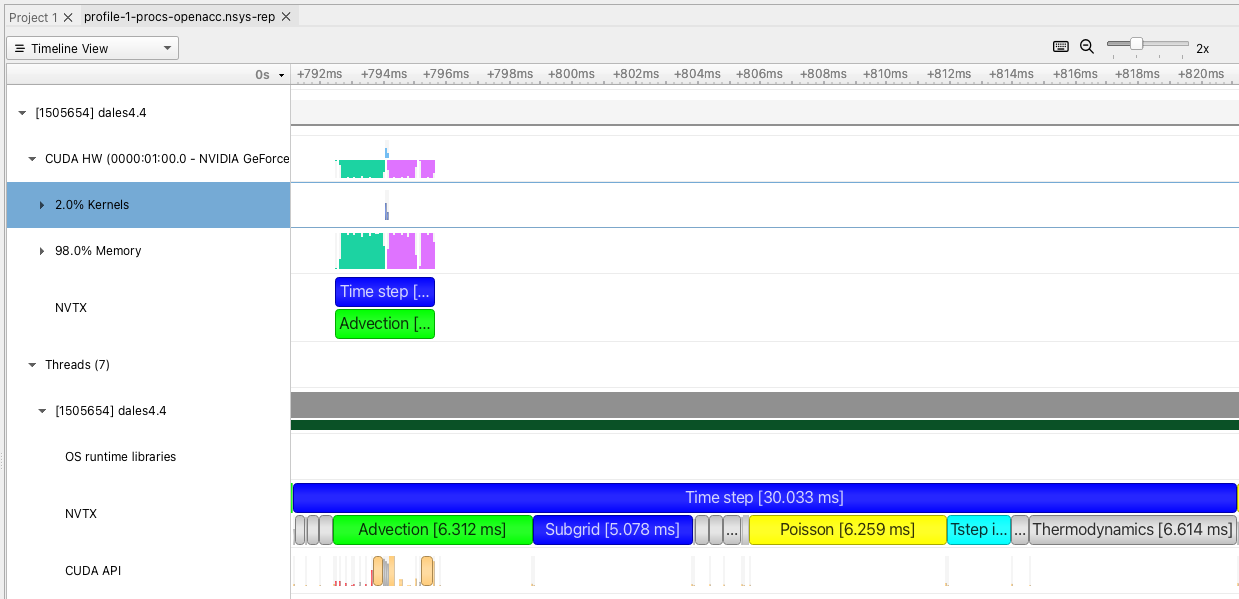
\includegraphics[width=0.9\textwidth]{doc/images/profiles/nsys.png}
    \caption{A screenshot of the NSys GUI. The main subroutine calls in DALES' time steps have been annotated with NVTX markers and show up at the bottom of the image, with their execution time between brackets. To demonstrate the GPU tracking capabilites of NSys, one advection kernel has been offloaded to the GPU (\texttt{advecu\_2nd}), which shows up under ``CUDA HW''. It can be seen that NSys automatically separates kernel execution time from time spent on memory operations, allowing for easy identification of performance bottlenecks.}
    \label{fig:nsys}
\end{figure}

\subsection{OpenACC}
As concluded from the literature, OpenACC is a relatively easy model to implement into an existing code base, while still offering good performance, given that data locality is properly optimized. Hence, the computationally expensive parts of DALES will be offloaded to the GPU using OpenACC. In \autoref{fig:nsys}, it can be seen that during one time step, most time is spent on the advection, sub-grid, Poisson and thermodynamics modules. These modules are expensive, because they consist mostly of loops that iterate over all grid points, making them also very well suited for offloading to GPUs with OpenACC. 

The first step in getting DALES running on GPUs, is to place OpenACC directives over all loops that are parallelizable. An example of a loop with an OpenACC directive can be found in \autoref{listing:accloop}. The offloading can be done loop-by-loop.
As mentioned multiple times before, memory transfers between CPU and GPU can make up a large portion of wall-clock time of an application. Hence, it is important to minimize the amount of data transfers, and optimize data locality (i.e., the location of data). When using OpenACC, the programmer does not have to be explicit about these data transfers, and let the compiler decide when to move data. To guarantee optimal data locality, is is good practice to explicitly copy data to and from the GPU. In OpenACC, this is also done via compiler directives. Data transfer will also be done manually in the OpenACC version of DALES. Ideally, all fields will be copied to the GPU before the time loop starts, and data will only be copied back to the CPU for writing output files with no additional data transfer in between. This may not be possible to realise for DALES, as some algorithms may be sequential by nature, meaning that they will not run efficiently on a GPU.

\begin{listing}[H]
\begin{minted}{fortran}
!$acc parallel loop collapse(3) default(present)
do k = 1, kmax
    do j = 1, jmax
        do i = 1, imax
            c(i,j,k) = a(i,j,k) + b(i,j,k)
        end do
    end do
end do
\end{minted}
\caption{Example of a Fortran loop decorated with an OpenACC directive. The directive \texttt{!\$acc parallel loop} tells the compiler that the following loop can be executed in parallel. The \texttt{collapse(3)} clause collapses the three nested loops into one big loop, exposing more parallelism, and the \texttt{default(present)} clause tells the compiler that the arrays \texttt{a}, \texttt{b} and \texttt{c} already exist on the GPU and no further data transfer is needed.}
\label{listing:accloop}
\end{listing}

\subsection{Solving the Poisson equation}

In DALES, a solution for the pressure $\pi$ is obtained by solving the following Poisson equation:

\begin{equation}
    \frac{\partial^2 \pi}{\partial x_i^2} = \frac{\partial }{\partial x_i} \left( - \frac{\partial \overline{u}_i \overline{u}_j}{\partial x_j} + \frac{g}{\theta_0}\overline{\theta}_v\delta_{i3} + \mathcal{F}_i - \frac{\partial \tau_{ij}}{\partial x_j} \right) \label{eq:pressure}
\end{equation}

 DALES provides two methods to solve this equation: using Fast Fourier Transforms (FFT's), or using iterative solvers. Among these, the FFT-based solver is the fastest. DALES has the ability to use the highly optimized Fastest Fourier Transform in the West (FFTW) library \citep{FFTW97}. FFTW is not capable of running on GPU's, however. NVIDIA provides a FFT library in their HPC SDK, which has a similiar interface as the FFTW library, making the conversion relatively straightforward.

\subsection{Multiple GPUs}
Currently, DALES is parallelized with MPI by decomposing the domain into slabs or pencils. On the other hand, OpenACC introduces further parallelization by distributing loop iterations among GPU threads. This means that MPI and OpenACC can be combined to run DALES on more than one GPU, for example by decomposing the domain into a number of chunks that equals the amount of available GPUs, and then binding each MPI process to a GPU. Communications do become even more expensive now, however, since a halo transfer would include copying the data from GPU to CPU, then from CPU to CPU, and from CPU to GPU again. Some of this performance penalty can be reduced by using an MPI implementations that is aware of GPU memory. 

The FFT-based Poisson equation solver relies very heavily on communication between processes (and therefore, GPUs). This is because it requires transposing the data in between FFT calculations, which in turn requires a redistribution of the data. Currently, the transpose operations are coded manually in DALES, using MPI \texttt{Alltoall} operations. When cuFFT is used, these transpose operations have to be adopted for the GPU as well. Alternatively, the multi-process version of cuFFT, cuFFTMp, can used. This library enables multi-process, multi-GPU FFTs, without the need to transpose the data and perform \texttt{MPI\_Alltoall} manually. In fact, inter-GPU communication is optimized using another communication library called NVSHMEM \citep{nvidiadeveloperNVSHMEM}, offering superior performance over regular MPI communications. The cuFFTMp library can bind to an existing MPI communicator, and transpose the data by itself when a 2D FFT is calculated. Yet another option is to use the cuDecomp library as described by \citet{romeroDistributedmemorySimulationsTurbulent2022}. cuDecomp does not offer any FFT functionality, but functions as an abstraction layer for the domain decomposition and communications. Given a number of MPI ranks, cuDecomp automatically determines the optimal domain decomposition (for example, given 32 processes, a 3D domain can be decomposed into 1$\times$32, 2$\times$16, or 4$\times$8 chunks, which do not necessarily yield the same performance). In addition, cuDecomp supports multiple communication backends (MPI, NVSHMEM, NCCL), from which it chooses the best performing during run time. This can improve performance significantly, especially when GPUs are distributed over multiple nodes. 

\subsection{Verification}
Modifying source code brings the possibility of introducing bugs in the code. While OpenACC requires minimal rewriting of source code, some rewriting may be inevitable. Hence, the updated source code needs to be validated against the original, unmodified code to check whether the program logic has changed. To this end, one would usually assert whether the end result of the two programs are equal or not. This approach is not feasible for a simulation of a turbulent boundary layer, however, as weather-like simulations are subject to chaos. A small perturbation of some prognostic variable can lead to vastly different results in the end. One source of such a perturbation can be the rounding off done by the computer. Even when using the exact same initial conditions, the point-wise end results of two runs may still differ, while each of the solutions could still be considered correct. A better approach would be to look at averaged statistics of several variables. 

